\subsection*{Træning}
Træningen er opdelt i tre boundarys. Boundaryen \textit{Evaluering} er først aktiv efter træningen, idet træningen skal evalueres. Der er til disse tre boundarys opstillet en fælles controller. Boundarys og controller fremgår af \autoref{fig:DesignTraening}. 

\begin{figure} [H]
\centering
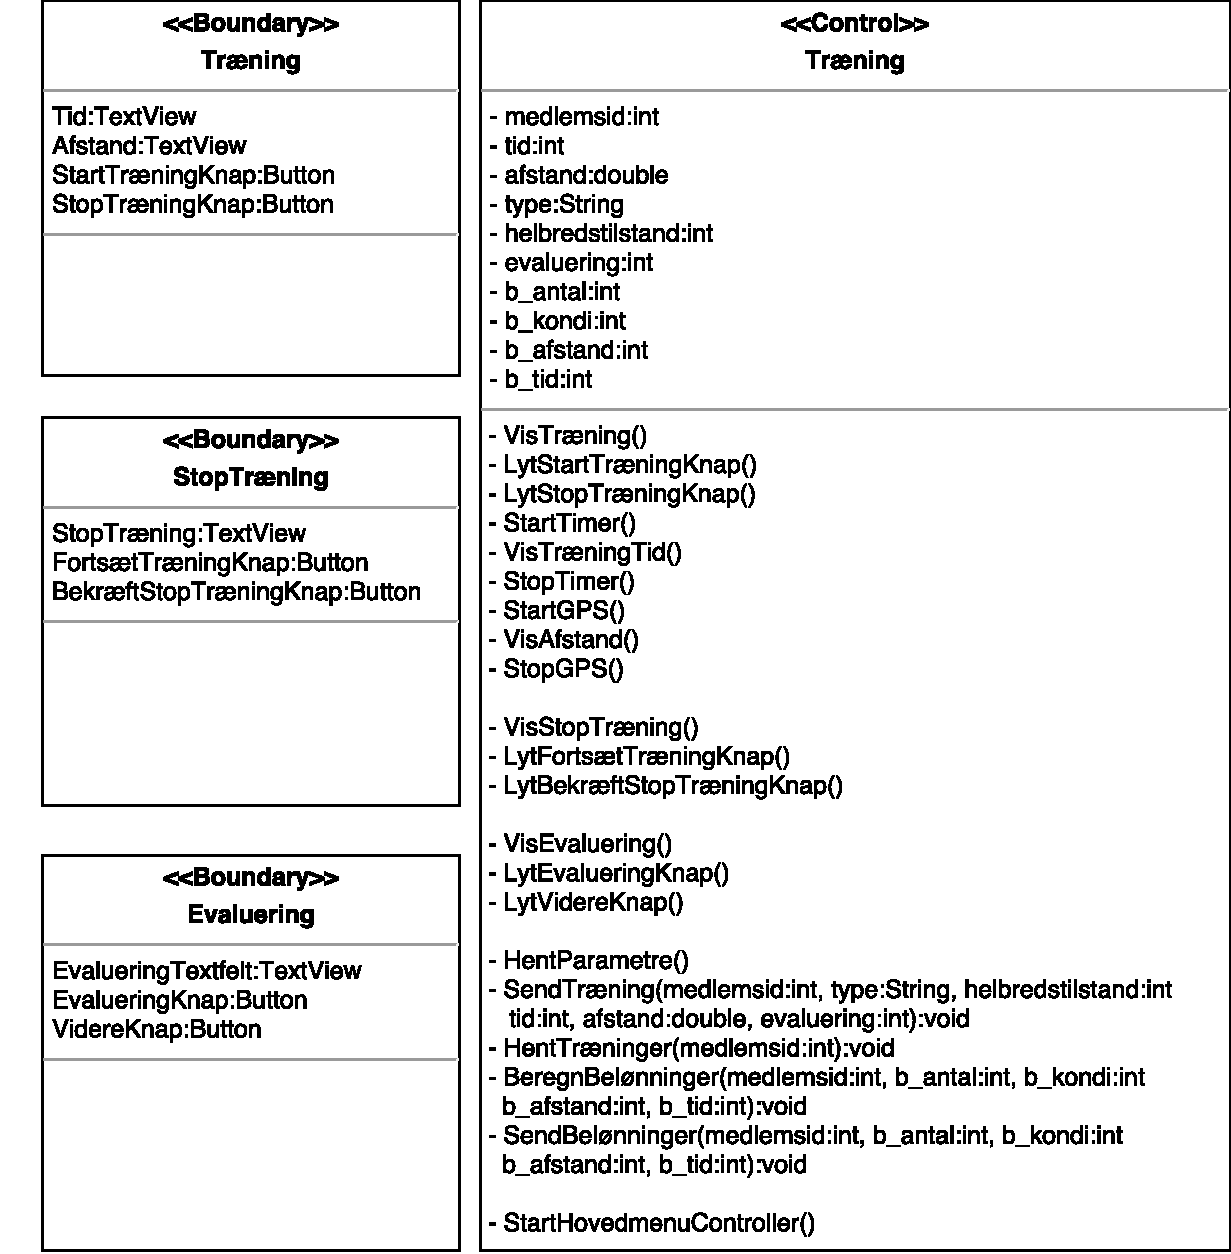
\includegraphics[width=0.7\textwidth]{figures/MVC/MVCTraening}
\caption{Designklasser for træning samt evaluering. Til venstre fremgår boundarys for Træning, StopTræning og Evaluering. Den tilhørende controller ses til højre.}
\label{fig:DesignTraening}
\end{figure}

\noindent
Grænsefladen for \textit{Træning}, \textit{StopTræning} og \textit{Evaluering} indeholder tekstfelter og knapper af typen TextView og Button. 


Controlleren \textit{Træning} indeholder private attributter samt metoder. Disse metoder omfatter Vis, Lyt, Start, Stop, Send, Hent og Beregn. Metoderne Send, Hent og Beregn handler i forhold til definerede inputsparametre.  

I sammenspil med designklasserne er der udarbejdet et sekvensdiagram, hvilket fremgår af \autoref{fig:SEKTraening}. 

\begin{figure} [H]
\centering
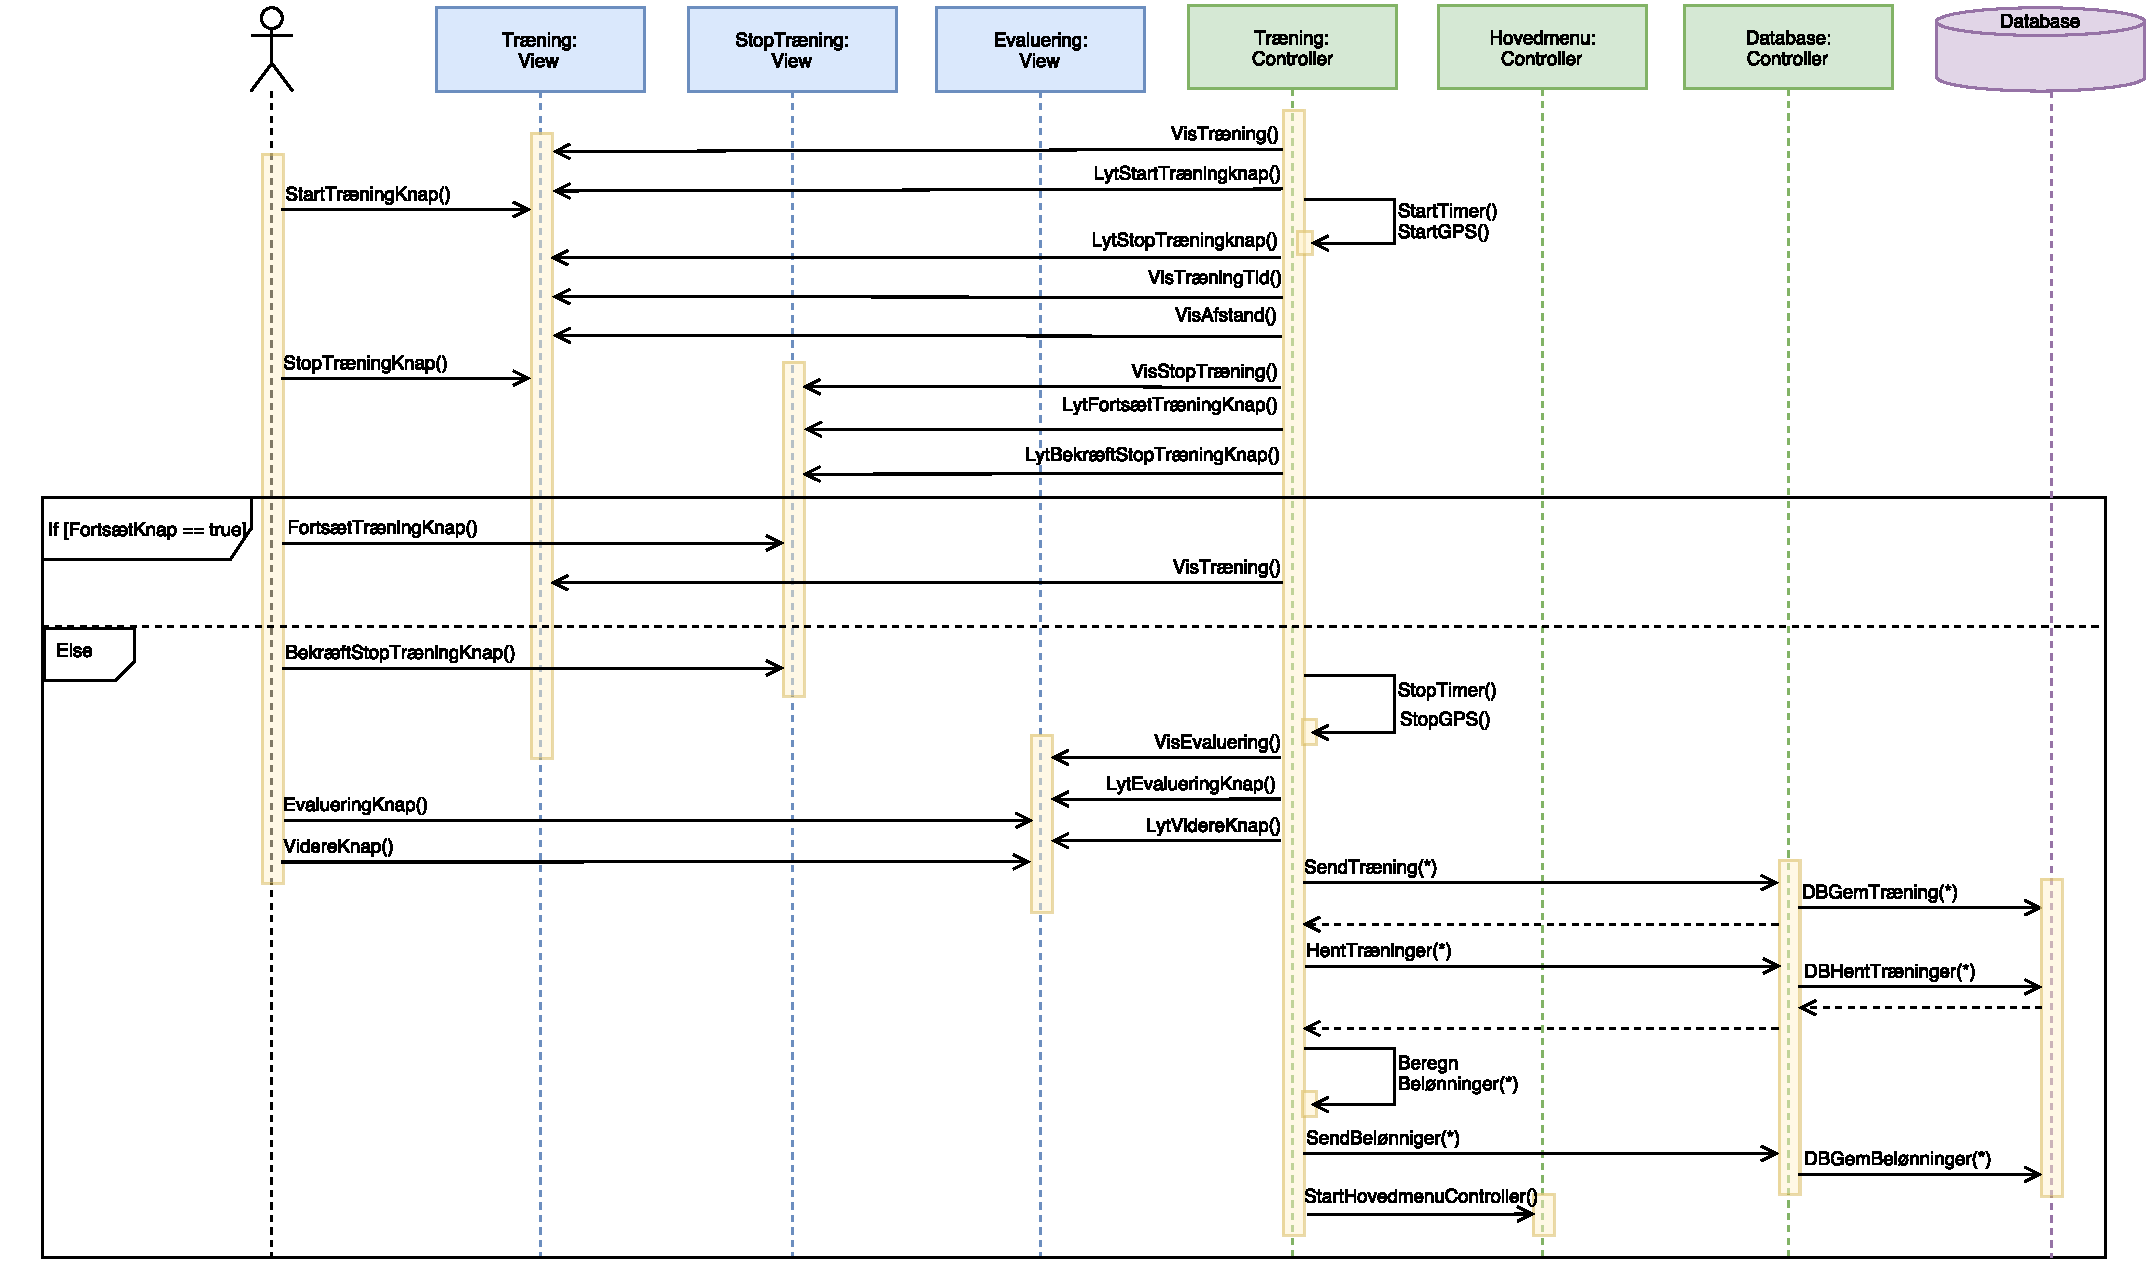
\includegraphics[width=1.55\textwidth, angle=90]{figures/Sek/SEKTraening}
\caption{Sekvensdiagram for træning.}
\label{fig:SEKTraening}
\end{figure}

\noindent
\textit{Træning} er den første grænseflade, der vises efter tilpasningen af træningsniveauet. Controlleren \textit{Træning} starter timer og GPS, når brugeren har trykket på StartTræningKnap. Herefter vises tiden og afstanden i grænsefladen. Brugeren kan under træningen, eller når træningen er fuldført, afslutte ved at trykke på StopTræningKnap, hvorefter grænsefladen for \textit{StopTræning} vises. I denne grænseflade har brugeren mulighed for at trykke på FortsætTræningKnap eller BekræftStopTræningKnap. Vælges FortsætTræningKnap vises grænsefladen for \textit{Træning}, og brugeren skal igen trykke på StartTræningKnap for at starte træning og måleenheder. Vælges BekræftStopTræningKnap stopper controlleren med at måle data fra GPS og timer. Herefter vises grænsefladen \textit{Evaluering}, hvor brugeren skal angive en evaluering af dagens træning. Evaluering bekræftes ved VidereKnap. Herefter sender controlleren træningsoplysninger til controlleren for \textit{Database}, som gemmer træningen i \textit{Database}. Stjerner indikerer, at metoden handler ud fra inputsparametre, hvilket fremgår af designklassen for tilhørende controller. Efterfølgende hentes tidligere træninger fra \textit{Database} via dens controller. Disse træninger benyttes for at beregnes brugerens samlede belønninger i \textit{Træning} controlleren. Derefter sendes disse til controlleren for \textit{Database}, der gemmer disse belønninger i \textit{Database} 
Derefter gives der besked til \textit{Hovedmenu} controlleren om at vise hovedmenuen.



%Denne indeholder tekstfelter, hvori tiden samt afstanden oplyses. Derudover er der et tekstfelt til kompatiblemålinger, hvis disse er tilsluttet. Da \textit{TræningsGrænsefladen} skal oplyse målinger fra tilkoblede kompatible måleenheder, skal denne grænseflade ligeledes styres af \textit{TilkoblingafkompatibleenhederController}, der ses af \autoref{fig:kompatiblemåleenheder}. Yderligere indeholder denne grænseflade en stopknap, af typen button, hvis træningen ønskes afsluttet. 
%Ønskes træningen afsluttet vises \textit{StopTræningGrænseflade}, hvori der er opstillet et tekstfelt samt to knapper. Tekstfeltet informerer brugeren om, at vedkommende er ved at afslutte træningen, hvorved brugeren kan bekræfte, at træningen skal stoppes eller fortsætte træningen ved hjælp af de opstillede knapper. 
%Efter en afsluttet træning, skal træningen evalueres, hvilket forekommer i \textit{EvalueringGrænsefladen}. Denne grænseflade indeholder et tekstfelt, der informerer brugeren om evalueringen, samt fire knapper. De tre knapper er opstillet således brugeren kan evaluere den udførte træning. Evalueringen bekræftes ved, at benytte den sidste knap til at bevæge sig videre i app’en. 
%\textit{TræningEvalueringController} er den fælles controller, som bestemmer, hvilken boundary, som vises. Denne controller lagrer tiden, afstanden, evaluering samt kompatible målinger, hvis disse er tilkoblet. Derudover lytter controlleren på de forskellige respektive knapper og håndterer skiftet mellem boundarys. Idet brugeren har evalueret sin træning og bekræftet ved at benytte videreknappen sendes alle træningsoplysningerne til databasen, hvori de gemmes. Dertil returneres brugeren til hovedmenuen. 
